\documentclass[conference]{IEEEtran}
\usepackage{cite}
\usepackage{balance}
\usepackage{amsmath}
\usepackage{graphicx}
\usepackage{booktabs}
\usepackage{array}
\usepackage{makecell}
\usepackage{textcomp}
\usepackage{url}
\newcommand{\rqRuns}{3}
\newcommand{\rqFullAcc}{97.894 $\pm$ 0.004}
\newcommand{\rqFullPrec}{91.93 $\pm$ 0.80}
\newcommand{\rqFullRec}{84.43 $\pm$ 0.55}
\newcommand{\rqFullFone}{86.42 $\pm$ 0.45}
\newcommand{\rqFullFpr}{0.245 $\pm$ 0.006}
\newcommand{\rqFullFnr}{5.787 $\pm$ 0.018}
\newcommand{\rqDedupAcc}{98.189 $\pm$ 0.011}
\newcommand{\rqDedupPrec}{83.15 $\pm$ 1.59}
\newcommand{\rqDedupRec}{76.78 $\pm$ 0.64}
\newcommand{\rqDedupFone}{78.78 $\pm$ 0.92}
\newcommand{\rqDedupFpr}{0.279 $\pm$ 0.004}
\newcommand{\rqDedupFnr}{6.908 $\pm$ 0.024}
\newcommand{\rqDupShare}{27.8}


\begin{document}

\title{Using Explanations to Diagnose a Dataset Shortcut in an Online Network Intrusion Detection System}

\author{\IEEEauthorblockN{Nguyen Thanh Son, Nguyen Tung Duong, Tang Khanh Nhi, and Vo Ngoc Bao Vy}
\IEEEauthorblockA{FPT University, Vietnam}}

\maketitle

\begin{abstract}
Intrusion detection systems based on machine learning are usually judged by accuracy on a public benchmark. We report a case in which a high score hid a shortcut. An XGBoost classifier trained on CSE-CIC-IDS2018, which we call M0, reaches 97.9\% accuracy on its test set, yet it raises an attack alert on 149 of 784 flows (19.0\%, 95\% CI 16.4 to 21.9) recorded on a Windows laptop and confirmed as benign. SHAP values, a decision-path trace, and tests that change one feature at a time point to the TCP FIN flag. A region defined by three conditions, the FIN zone, holds 148 of the 149 alerts on the live flows and 99.97\% of the false alerts on a large labeled benign test set. In the original training data this region holds only DoS-Hulk flows. The pattern fits an extractor that ended flows at the first FIN packet, as earlier work reports for related datasets, but we could not check this on raw packets. A second classifier, M1, trained in the same way on recreated data with corrected labels, raises no alert on the 784 flows (95\% upper bound 0.47\%). The corrected benchmark contains near-duplicate flows, so its 99.99\% accuracy does not predict field performance. With the kernel width of our earlier study, LIME gave no valid local fit on real flows, and wider kernels pass the quality gate only by making the fit nearly global, while TreeSHAP passed the additivity check on every flow.
\end{abstract}

\begin{IEEEkeywords}
intrusion detection, explainable artificial intelligence, SHAP, LIME, XGBoost, dataset quality, shortcut learning
\end{IEEEkeywords}

\section{Introduction}
A machine-learning intrusion detection system is usually trained and tested on one public dataset, and the test accuracy is taken as the measure of quality. CSE-CIC-IDS2018 \cite{sharafaldin2018} is one of the datasets used this way. Liu et al.\ describe it as a primary benchmark for network intrusion detection \cite{liu2022}. The same authors, and Engelen et al.\ before them, found errors in how these datasets were built \cite{engelen2021,liu2022}. A practitioner who trains on such data cannot tell from the test score whether an error has entered the model.

We met this problem while building an online detector. The work followed four research questions, and each question builds on the answer to the one before.
\begin{itemize}
\item \textbf{RQ1.} How well does an XGBoost classifier \cite{chen2016} detect attacks on CSE-CIC-IDS2018? The resulting model is called M0.
\item \textbf{RQ2.} Which explanation method, SHAP \cite{lundberg2017,lundberg2020} or LIME \cite{ribeiro2016}, suits this detector?
\item \textbf{RQ3.} Can the detector and its explanations run in an online system, and how does the detector behave on real traffic?
\item \textbf{RQ4.} Can explanations trace a failure seen in RQ3 to a shortcut in the training data, and does retraining on corrected data remove the failure? The retrained model is called M1.
\end{itemize}

The answers form one story, and each result leads to the next question. In RQ1, M0 scored 97.9\% accuracy, so we kept it. A label alone does not tell an analyst why a flow was flagged, so RQ2 compared explainers, and SHAP proved the better one. We then deployed M0 with SHAP in RQ3, and it raised attack alerts on benign traffic from our own laptop, which the benchmark score had not predicted. RQ4 asks why. SHAP and a trace of the decision path identified a likely data shortcut, and retraining on corrected data removed the observed false-alert pattern. Fig.~\ref{fig:chain} shows the chain of evidence.

M0 is the detector that failed. It is trained on the original data. M1 uses the same algorithm, the same settings, and the same sampling recipe, and it is trained on a corrected version of the same dataset \cite{liu2022}. We train M1 for one reason, which is to test the explanation. If the shortcut comes from the training data, a model trained on corrected data should not show it. If M1 still raised alerts on the same traffic, the cause would lie elsewhere, for example in the features or in the live traffic. Between M0 and M1, the algorithm and the settings stay the same, and the training data change in the extractor, the labels, and the class set.

The paper makes three contributions.
\begin{itemize}
\item It documents a case in which a shortcut in a public intrusion dataset gives a 19\% alert rate on confirmed-benign traffic, while the benchmark accuracy is 97.9\%.
\item It shows a short diagnostic procedure made of SHAP values, a decision-path trace, a region test on later data, feature-intervention sensitivity tests, and a check of the training data.
\item It checks the fix and reports its limits. The retrained model raises no alert on the confirmed-benign flows, but its benchmark is easy, LIME gave a valid fit on real flows only with kernels so wide that the fit is no longer local, and the system works at the level of completed flows.
\end{itemize}

\begin{figure*}[t]
\centering
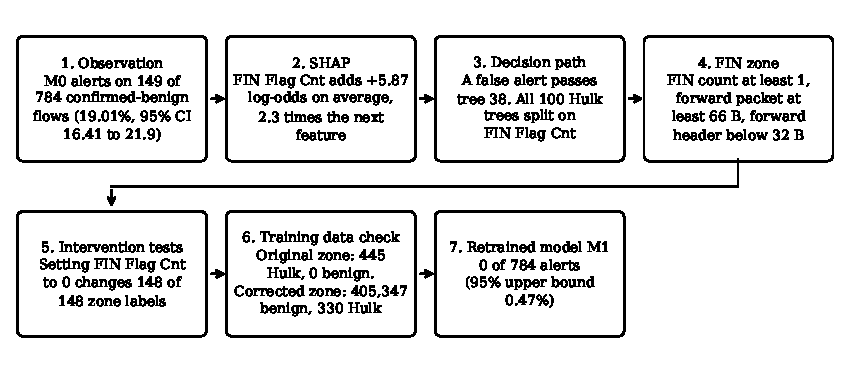
\includegraphics[width=0.92\textwidth]{figures/fig1_chain.pdf}
\caption{Chain of evidence in this paper. Steps 1 to 3 and 5 use the 784 live flows or the 148 flows of the FIN zone among them. Step 4 is validated on later data, and step 6 uses the training sets. Step 7 uses the 784 live flows again, with M1.}
\label{fig:chain}
\end{figure*}

\section{Related Work}
\subsection{Quality of the CIC datasets}
CSE-CIC-IDS2018 was produced by the Communications Security Establishment and the Canadian Institute for Cybersecurity from a laboratory network with scripted attacks \cite{sharafaldin2018}. Engelen et al.\ examined the earlier CIC-IDS-2017 data. They report that the flow extractor ends a flow at the first FIN packet, so the last packets of a connection become separate flows, and that some labels do not match the traffic \cite{engelen2021}. Liu et al.\ extended the study to CSE-CIC-IDS2018. They report errors in attack orchestration, feature generation, documentation, and labeling, and they publish recreated datasets with corrected labels and a fixed flow extractor \cite{liu2022}. These studies document the errors. They do not follow an error into a trained and deployed model, which is the question we study.

\subsection{Pitfalls of machine learning in security}
Sommer and Paxson discuss why machine learning has seen little operational use in network intrusion detection and describe the evaluation problems that follow \cite{sommer2010}. Arp et al.\ review 30 papers from top security conferences and show that common pitfalls can inflate reported results \cite{arp2022}. Geirhos et al.\ describe shortcut learning, in which a model adopts a strategy that succeeds on a benchmark but fails under realistic conditions \cite{geirhos2020}. The FIN pattern in this paper is a shortcut of that kind in a tabular intrusion detector.

\subsection{Explanations for intrusion detection}
SHAP assigns each feature a share of one prediction \cite{lundberg2017}, and its tree version computes these shares exactly for tree ensembles \cite{lundberg2020}. LIME fits a simple model to the classifier around one input \cite{ribeiro2016}. Neupane et al.\ survey explainable intrusion detection and call for metrics that evaluate explanations \cite{neupane2022}. Marino et al.\ explain misclassifications on NSL-KDD by searching for the smallest feature changes that correct them \cite{marino2018}. Warnecke et al.\ propose criteria for comparing explanation methods in security tasks \cite{warnecke2020}. Slack et al.\ show that explanations built from perturbed inputs can be unreliable \cite{slack2019}, and Alvarez-Melis and Jaakkola propose to measure whether similar inputs receive similar explanations \cite{alvarezmelis2018}. These works compare explanation methods or propose new ones. We use explanations for a different purpose. We look for the reason a classifier fails on real traffic, and then we test that reason on later data.

\section{Data and Models}
\subsection{Original data and model M0}
Our input is ten daily cleaned Parquet files derived from the processed CSV files of CSE-CIC-IDS2018, with 78 features per flow and 15,589,784 flows in total. A sample of 3.5 million flows, drawn by class, was split 80/20 into 2,800,000 training flows and 700,000 test flows, with the same class shares in both parts. The data have 15 classes, one benign class and 14 attack classes. Model M0 is an XGBoost classifier with 100 trees, depth 8, learning rate 0.08, and the histogram tree method, with seed 42.

\subsection{Retrained model M1 and the two data domains}
Liu et al.\ rebuilt the flows from the original packet captures with a fixed extractor and recomputed the labels from IP addresses, ports, payload, and time \cite{liu2022}. We call these recreated flows the corrected data, because they come from a fixed extractor and carry corrected labels. We trained M1 on these flows with the same hyperparameters and the same class-wise sampling recipe. M1 has 13 classes and uses 2,728,397 training flows and 682,100 test flows.

M0 and M1 therefore learn from two different data domains. The domains differ in the flow extractor, in the labels, and in the class set, as Table~\ref{tab:data} shows. Because the extractor and the labels change together, our test of the data as the cause cannot separate the two. A score of one model on the other domain would mix model quality with domain differences. We do not report such transfer results, and we use the two models side by side only on benign flows, where the correct answer is the same in both domains. We do not report M1 on the original test set, and we make no claim about transfer between the domains.

\begin{table}[t]
\caption{What differs between the two training domains. The extractor row states what earlier work reports and what we could not check.}
\label{tab:data}
\centering
\footnotesize
\setlength{\tabcolsep}{3pt}
\begin{tabular}{>{\raggedright\arraybackslash}p{0.95in}>{\raggedright\arraybackslash}p{1.15in}>{\raggedright\arraybackslash}p{1.15in}}
\toprule
Item & Original data (M0) & Corrected data (M1) \\
\midrule
Source & Processed CSV files of CSE-CIC-IDS2018 & Recreated by Liu et al.\ from the original captures \\
Flow extractor & Original CICFlowMeter, reported to end flows at the first FIN in related data, not checked by us & Fixed CICFlowMeter of Liu et al. \\
Labels & Original labeling & Recomputed from IP, port, payload, and time \\
Training and test flows & 2,800,000 and 700,000 & 2,728,397 and 682,100 \\
Classes & 15 & 13 \\
Test rows also in training set & 27.7\% (194,149 of 700,000) & 16.9\% (115,467 of 682,100) \\
Flows with at least 4 packets each way that carry FIN & 0.065\% (428 of 661,302) & 70.9\% (1,179,170 of 1,662,550) \\
Benign and Hulk flows in the FIN zone & 0 and 445 & 405,347 and 330 \\
\bottomrule
\end{tabular}
\end{table}

\subsection{Live traffic and lab flows}
\textit{Live set.} The 784 live flows come from four capture sessions on one Windows laptop on 22 October 2026, between 12:40 and 14:01 UTC. The system captured packets on the laptop and recorded 45, 36, 478, and 477 flows in the four sessions. We kept the flows that have one of two laptop addresses at one end, which are the addresses of the home Wi-Fi network and of a phone hotspot, and we removed multicast and broadcast flows. This left 34, 32, 242, and 476 flows. We confirmed verbally on 26 October 2026 that no attack ran during the sessions. We kept no activity log, so the benign label rests on this statement alone. The set was built after the FIN zone was defined, as Section~\ref{sec:zone} explains.

\textit{Lab flows.} In a lab of two virtual machines on one host we captured one file of web browsing, with 21 flows, and two files of SSH brute-force traffic, with one flow in each file. The lab operator assigned the labels. Each SSH file holds one connection that lasted 21.2 s and 57.3 s. We use these two flows only as a check of the retrained model, as Section~\ref{sec:m1} explains.

\section{RQ1: Detection Performance of M0}
\textit{Why we ask.} Every later step needs a detector, so we first measure how well a classifier trained on the original data detects attacks.

\textit{Setup.} We scanned seven XGBoost configurations and kept the one in Section~III-A. The test set served for this choice, so the reported scores are somewhat optimistic. In an earlier report, a Random Forest tuned by a randomized search (80 trees, depth 28) had about 5 points lower macro F1 and about 12 points lower macro precision than XGBoost, and about 2 points higher macro recall. We did not rerun that comparison, and we have no verified false-positive rate for the Random Forest, so we make no claim about it. We chose XGBoost for its higher macro F1 and precision. TreeSHAP also gives exact explanations for tree ensembles.

\textit{Result.} M0 reaches 97.91\% accuracy, 85.81\% macro F1, a benign alert rate of 0.23\%, and a false-negative rate of 5.75\% on its test set. To check how much these numbers depend on one split, we pooled the 3.5 million flows, split them again three times with different seeds, and retrained the model each time. Table~\ref{tab:rq1} gives the means and standard deviations. We also scored each retrained model on the part of its test set whose feature vectors do not occur in its training set. Across the three splits, \rqDupShare\% of the test rows also appear in the training set. The three retrained models reach 97.89\% accuracy on average, which matches the 97.91\% of M0. Their macro F1 is 0.3 to 1.1 points higher than the 85.81\% of M0, so M0 sits at the low end of the range that different splits produce. Removing the duplicated rows lowers macro F1 by about 7.6 points and leaves accuracy near 98\%. Part of the macro F1 on the full test set therefore comes from flows that the model has already seen in training.

\begin{table}[t]
\caption{Three stratified re-splits of the original data. Values are mean $\pm$ standard deviation, in percent. The benign alert rate is the share of benign flows that receive any attack label.}
\label{tab:rq1}
\centering
\small
\begin{tabular}{lcc}
\toprule
Metric & Full test set & Without duplicates \\
\midrule
Accuracy & \rqFullAcc & \rqDedupAcc \\
Macro precision & \rqFullPrec & \rqDedupPrec \\
Macro recall & \rqFullRec & \rqDedupRec \\
Macro F1 & \rqFullFone & \rqDedupFone \\
Benign alert rate & \rqFullFpr & \rqDedupFpr \\
False-negative rate & \rqFullFnr & \rqDedupFnr \\
\bottomrule
\end{tabular}
\end{table}

\textit{Answer to RQ1.} M0 detects attacks well on its own benchmark. The score includes flows seen in training, so it is an upper estimate. We keep M0 for the next steps. A detector that only returns a label gives an analyst no reason to trust the alert, and this leads to RQ2.

\section{RQ2: SHAP Versus LIME}
\textit{Why we ask.} An analyst who receives an alert needs to know which features drove it. Two methods are widely used for this, SHAP and LIME, and the system can serve only one of them for every alert, so we had to choose.

\textit{Setup.} We compared the two explainers on 1,339 flows of the original test set, at most 100 per class. We used LIME with a kernel width of 3.312, 1,000 perturbed samples, and a background of 2,000 training flows. We measured agreement of the top five features, faithfulness by deleting the top features and watching the predicted probability fall, stability across ten random seeds, and stability under input noise. We also applied a quality gate to LIME, a local fit of $R^2\ge 0.3$, a threshold we set ourselves.

\textit{Result.} Table~\ref{tab:xai} gives the results. The top features of the two methods overlap little, with a Jaccard index of 0.141 at five features, against 0.036 for random rankings. SHAP lowers the predicted probability more than LIME for 78\% of flows (Wilcoxon signed-rank test, $p<10^{-140}$). SHAP is deterministic, while LIME gives different rankings across seeds. On the 1,339 flows, 85.96\% of the LIME explanations pass the quality gate, but only 23\% of the 100 benign flows do.

\begin{table}[t]
\caption{SHAP and LIME on 1,339 flows of the original test set.}
\label{tab:xai}
\centering
\small
\begin{tabular}{lcc}
\toprule
Measure & SHAP & LIME \\
\midrule
Faithfulness, area under deletion curve & 0.81 & 0.46 \\
Faithfulness of random ranking & \multicolumn{2}{c}{0.11} \\
Stability across 10 seeds, Jaccard at 5 & 1.00 & 0.58 \\
Jaccard at 5 under 10\% noise & 0.46 & 0.18 \\
\bottomrule
\end{tabular}
\end{table}

\textit{Answer to RQ2.} SHAP is more faithful and more stable than LIME on this detector, and it is less sensitive to noise. The online system therefore computes SHAP values for every alert and runs LIME only on request. With a detector and an explainer chosen, the next step is to use them the way an analyst would, which is RQ3.

\section{RQ3: The Online System and Its First Deployment}
\textit{Why we ask.} Scores on a test set do not show how a detector behaves on traffic that nobody labeled for it. We therefore built a system that receives packets, builds flows, classifies them, and explains the alerts, and we ran it on our own traffic.

\subsection{System design}
Fig.~\ref{fig:pipeline} shows the pipeline. Scapy reads packets through the Npcap driver on Windows or from a PCAP file. A flow extractor based on CICFlowMeter groups packets into flows and computes the 78 features. Our extractor closes a TCP flow only after both directions have sent a FIN that the other side acknowledged, or on a reset, a timeout, or a new SYN from the same address pair. A feeder process sends each flow to a REST API, which validates the 78 features, runs the XGBoost classifier, and stores the result in SQLite.

For every alert, meaning every flow that receives an attack label, the system computes TreeSHAP values in a background queue. LIME runs only when the analyst asks for it. Two flags mark explanations that need care. The environment flag is raised when at least two of the five strongest SHAP features belong to a set of four features that depend on the operating system or the lab setup. These are the destination port, the minimum forward header size, the initial forward window size, and the FIN flag count. The rare-class flag is raised when the predicted class has fewer than 100 training flows. The flags only change how the dashboard displays an alert. We did not validate them as measures of explanation quality.

\begin{figure*}[t]
\centering
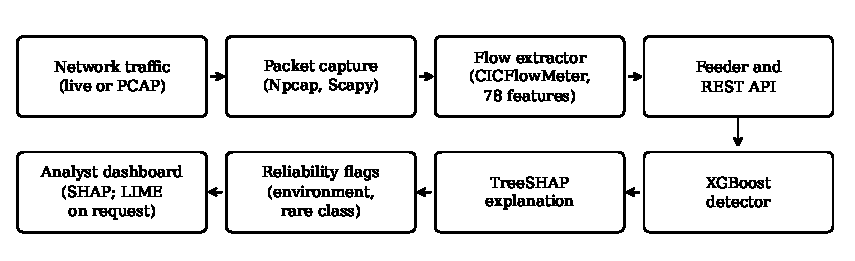
\includegraphics[width=0.92\textwidth]{figures/fig2_pipeline.pdf}
\caption{The online system. LIME runs only on the analyst's request.}
\label{fig:pipeline}
\end{figure*}

\subsection{Processing time and delay}
Fig.~\ref{fig:latency} shows the processing times for 1,025 flows and 219 alerts in a lab session that mixed CSV upload, PCAP replay, and live capture. The median time was 2.5 ms for validation, 12.4 ms for classification (95th percentile 22.4 ms), 32.5 ms for the SHAP values (40.3 ms), and 26.7 ms for the flags. The whole request took a median of 19.3 ms and at most 252.6 ms. SHAP tasks waited in the queue for a median of 2.2 s and at most 5.8 s, because 219 alerts arrived in a burst, mostly from one CSV upload.

The system works at the flow level. A flow is classified after the extractor closes it. In the 290 flows of a live session, the median flow lasted 1.35 s, the 90th percentile 49.0 s, and the longest 89.9 s. Detection delay is therefore dominated by flow duration and not by processing, and we call the system online and not real-time.

\begin{figure}[t]
\centering
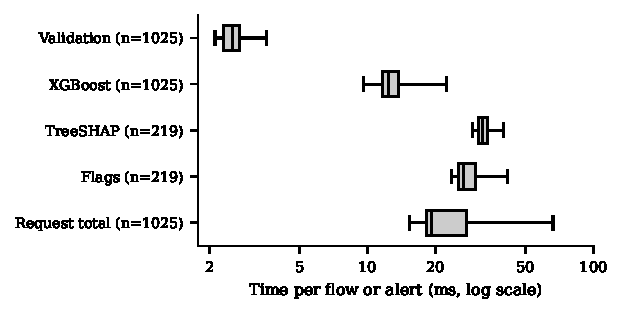
\includegraphics[width=\columnwidth]{figures/fig7_latency.pdf}
\caption{Processing time per flow or alert. Boxes show the quartiles and whiskers the 5th and 95th percentiles.}
\label{fig:latency}
\end{figure}

\subsection{First deployment of M0 on live traffic}
We ran M0 on the 784 live flows. M0 raised an attack alert on 149 flows, a rate of 19.01\% (95\% Wilson interval 16.41 to 21.90). Of these alerts, 148 carry the DoS-Hulk label. The alert rate differs between the four sessions, from 11\% to 59\%, and flows within a session are not independent, so the interval understates the uncertainty. On the 21 lab flows of web browsing, M0 raised an alert on 19. These flows are benign, so every alert is a false one, and the benchmark score of 97.9\% gave no warning of it.

\subsection{Explanations on live flows}
TreeSHAP values passed the additivity check on all 784 live flows. The sum of the SHAP values and the base value matched the raw model output with a largest absolute error of $4.8\times 10^{-6}$ for M0. This checks the arithmetic of the explanation. It does not show that the explanation helps an analyst.

LIME behaved differently. We ran it on 313 real flows, made of the 290 flows of one live session, the 21 browsing flows, and the two SSH flows. With M0 and the original background, 255 flows have an effective sample size below two, which means that almost no perturbed sample lies near the flow, and only three flows reach the quality gate. We tested two possible remedies in RQ4, once the retrained model was available.

\textit{Answer to RQ3.} The detector and its explanations run online, with a median of 12.4 ms to classify a flow and 32.5 ms to compute SHAP values, but detection is delayed by flow duration. The deployment exposed a failure of M0. It raised alerts on 19.0\% of confirmed-benign live flows, and LIME gave no valid fit on most of them. RQ4 looks for the cause.

\section{RQ4: Tracing the Failure to the Data and Testing a Fix}
\textit{Why we ask.} RQ3 showed that M0 flags benign traffic, a result that the benchmark score of RQ1 did not predict. The alerts are a symptom. We therefore ask where they come from, and whether the training data are the cause.

\subsection{SHAP points to one feature}
To see what drives the alerts, we explain them with SHAP, which RQ2 selected. We computed TreeSHAP values of the DoS-Hulk output for the 148 live flows that M0 labeled as Hulk. Fig.~\ref{fig:shap}a shows the mean values. The FIN flag count contributes 5.87 log-odds units on average, which is more than twice the next feature, the largest forward packet at 2.60. The other six of the eight strongest features contribute less than 0.6 each in absolute value. Fig.~\ref{fig:shap}b shows the same quantity for M1, which Section~\ref{sec:m1} discusses.

\begin{figure*}[t]
\centering
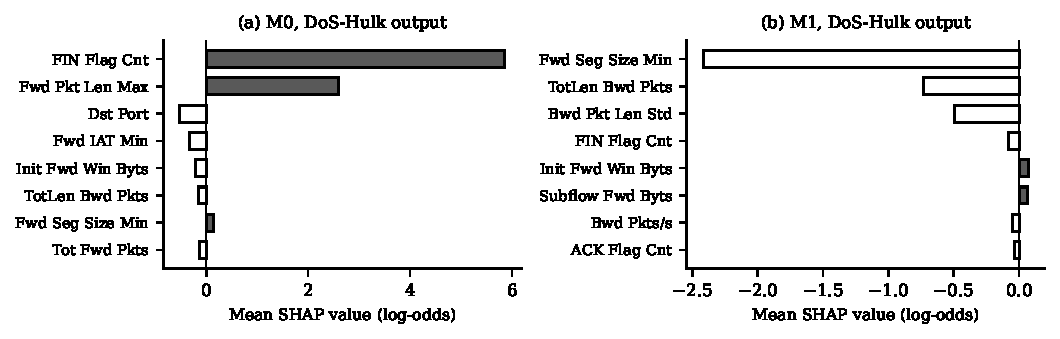
\includegraphics[width=0.92\textwidth]{figures/fig4_shap.pdf}
\caption{Mean SHAP value of the DoS-Hulk output over the same 148 live flows in the FIN zone, for (a) M0 and (b) M1. M0 labels all 148 flows as Hulk, and M1 labels all 148 as benign.}
\label{fig:shap}
\end{figure*}

\subsection{Decision path and the FIN zone}
\label{sec:zone}
SHAP gives a mean contribution for each feature, but it does not describe a region of the feature space. We want a rule that we can test on other data, so we traced the decision path of one alert.

\textit{How the zone was defined.} On 18 October 2026, one false DoS-Hulk alert from a live session had a Hulk probability of 93.3\%. We traced its path through the 100 trees of the Hulk class. All 100 trees contain at least one split on the FIN flag count. In the tree with the highest gain, tree number 38, the path of the alert passes three tests in order. The minimum forward header size is below 32 bytes, the FIN count is at least one, and the largest forward packet is at least 66 bytes. We call the set of flows that satisfy all three tests the FIN zone. We described the three conditions in the project documentation the same day and added them to the system configuration on 20 October. They come from one false alert and one tree, and not from a search over data.

\textit{Validation on later data.} A rule built from one alert could be chance, so we tested it on data collected afterwards. The 784 live flows were captured four days after the zone was defined and two days after it entered the configuration, and the corrected-label test set was prepared later still. Neither set was used to choose the three conditions. Table~\ref{tab:zone} shows the result. In the live set, all 148 flows in the zone received an attack label, and 148 of the 149 alerts lie in the zone. This holds in each of the four sessions. In the labeled benign test set, 100,817 of 100,849 alerts lie in the zone, which is 99.97\%, and 100,817 of the 100,819 benign flows in the zone raised an alert. The three conditions therefore describe almost all false alerts of M0 on both sets.

\begin{table}[t]
\caption{Alerts of M0 on benign flows and their position relative to the FIN zone.}
\label{tab:zone}
\centering
\footnotesize
\setlength{\tabcolsep}{3pt}
\begin{tabular}{lrrrr}
\toprule
Set & Flows & In zone & Alerts & \makecell[r]{Alerts\\in zone} \\
\midrule
Session 1 & 34 & 19 & 20 & 19 \\
Session 2 & 32 & 19 & 19 & 19 \\
Session 3 & 242 & 27 & 27 & 27 \\
Session 4 & 476 & 83 & 83 & 83 \\
Live, all & 784 & 148 & 149 & 148 \\
\midrule
Labeled test & 477,470 & 100,819 & 100,849 & 100,817 \\
\bottomrule
\end{tabular}
\end{table}

\subsection{Feature-intervention sensitivity tests}
Large SHAP values show where the model looks, but they do not show that the labels depend on that feature. We therefore changed one feature at a time on the 784 live flows and counted the flows whose label changed. These tests measure how sensitive the model is to one feature. They do not describe flows that real traffic would produce, because a changed flow may not occur in practice. They are not evidence of cause in real traffic. Table~\ref{tab:interv} gives the results. Setting the FIN count to zero changes the label of all 148 zone flows, and only four alerts remain. Setting the largest forward packet to zero also changes all 148 labels. Setting the minimum forward header to 32 bytes changes 165 labels. Two controls, the initial forward window set to 64,240 bytes and the destination port set to 80, change 1 and 5 labels. The three zone conditions therefore carry the decision, and two unrelated features do not.

\begin{table}[t]
\caption{Feature-intervention tests of M0 on the 784 live flows. M0 raises 149 alerts before any change.}
\label{tab:interv}
\centering
\footnotesize
\setlength{\tabcolsep}{3pt}
\begin{tabular}{lrr}
\toprule
Change applied to all flows & \makecell[r]{Labels\\changed} & \makecell[r]{Alerts\\left} \\
\midrule
FIN Flag Cnt = 0 & 148 & 4 \\
Fwd Pkt Len Max = 0 & 148 & 3 \\
Fwd Seg Size Min = 32 & 165 & 22 \\
\midrule
Init Fwd Win Byts = 64,240 (control) & 1 & 148 \\
Dst Port = 80 (control) & 5 & 148 \\
\bottomrule
\end{tabular}
\end{table}

\subsection{What the training data show}
If M0 depends on the zone, its training data must have taught it, so we looked at what the training data contain in the zone. Fig.~\ref{fig:zone} gives the number of flows in the FIN zone in the two training sets. In the original training set the zone holds 445 flows, and all are DoS-Hulk. For M0 the zone is a perfect signal of that class. FIN alone is not the whole rule. The original training set has 9,815 benign flows with a nonzero FIN count, but none of them lies in the zone. In the corrected training set the same zone holds 405,347 benign flows and 330 Hulk flows. It also holds flows of other attack classes, for example 238,320 HOIC flows and 100,650 Bot flows, so the zone no longer identifies Hulk in that set.

A difference in FIN frequency fits this picture. Among original training flows with at least four packets in each direction, only 0.065\% carry a FIN flag, 428 of 661,302. In the corrected training set, 70.9\% of such flows do. Earlier work reports that the original extractor ends a flow at the first FIN packet in CIC-IDS-2017 \cite{engelen2021}, and the documentation of the corrected data states that the Hulk attack in CSE-CIC-IDS2018 shows the same behavior \cite{liu2022}. Our results fit this hypothesis, but we did not check it on raw packets, which we do not have. We treat the extractor as the likely cause and not as a proven one.

\begin{figure}[t]
\centering
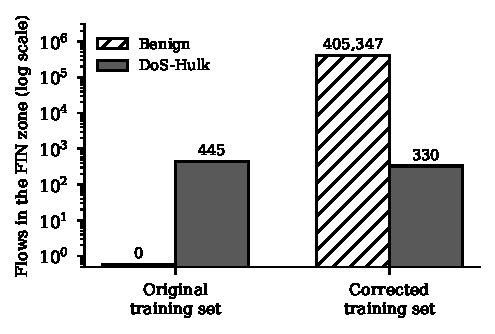
\includegraphics[width=\columnwidth]{figures/fig3_zone.pdf}
\caption{Number of benign and DoS-Hulk flows in the FIN zone in the two training sets. The corrected set also has flows of other attack classes in the zone. The original set has no benign flow in the zone, and this zero is drawn at the bottom of the logarithmic axis.}
\label{fig:zone}
\end{figure}

\subsection{Retraining on the corrected data}
\label{sec:m1}
The training data point to the data as a likely cause. To test this, we trained M1 on the corrected data, which has a different extractor, different labels, and a different class set, while the algorithm and the settings stay the same. This is the test of the explanation, but it cannot tell which of the three differences matters. We measured the alert rate of both models on three sets of benign flows. The first is the benign part of the corrected-label test set, with 477,470 flows. The second is the 784 live flows. The third is the 21 lab flows of web browsing. Table~\ref{tab:alert} gives the results. Intervals are 95\% Wilson intervals, and the upper bound for zero alerts is the Clopper-Pearson bound. M0 raises an alert on 21.12\% of the labeled benign test flows, against 0.23\% on its own test set. M1 raises 7 alerts on the labeled benign test flows and none on the live and browsing flows.

\begin{table*}[t]
\caption{Alert rate on benign flows, with 95\% confidence intervals. M0 is trained on the original data and M1 on the corrected data.}
\label{tab:alert}
\centering
\small
\begin{tabular}{lrcc}
\toprule
Benign set & Flows & M0 alerts (rate, interval) & M1 alerts (rate, interval) \\
\midrule
Labeled test flows, corrected labels & 477,470 & 100,849 (21.12\%, 21.01 to 21.24) & 7 (0.0015\%, 0.0007 to 0.0030) \\
Live traffic, confirmed benign & 784 & 149 (19.01\%, 16.41 to 21.90) & 0 (0.00\%, upper bound 0.47) \\
Lab web browsing & 21 & 19 (90.48\%, 71.09 to 97.35) & 0 (0.00\%, upper bound 16.11) \\
\bottomrule
\end{tabular}
\end{table*}

All 148 live flows in the FIN zone receive the benign label from M1. Fig.~\ref{fig:shap}b shows why. For the Hulk output of M1, the FIN count contributes only $-0.08$ on average, and the strongest feature is the minimum forward header size, with $-2.42$, which pushes the decision away from Hulk. M1 uses a different feature in place of FIN, and that feature also depends on the operating system.

\textit{Benchmark score of M1.} M1 reaches 99.996\% accuracy and 99.30\% macro F1 on its random-split test set. This is higher than any score of M0, and a score this high calls for a check, because it could come from duplicates or from an easy split. We checked this score with a time-blocked split, a duplicate count, and simple baselines. For the time-blocked split, we cut each class into five contiguous time blocks, trained on four blocks with a 1\% gap at both ends of the test block, and tested on the fifth (Fig.~\ref{fig:blocked}). Macro F1 ranges from 98.1\% to 99.99\% over the blocks, and the benign alert rate from 0.0015\% to 0.0034\%. In the random split, 115,467 of the 682,100 test rows, 16.9\%, also occur in the training set, and removing them leaves accuracy at 99.996\%. On this data, a classifier that always answers benign reaches 70.0\% accuracy, a decision tree of depth three reaches 96.4\%, and a model trained on 0.1\% of the training data reaches 99.76\% accuracy and 96.63\% macro F1. The benchmark is easy. Its score does not predict field performance.

\begin{figure}[t]
\centering
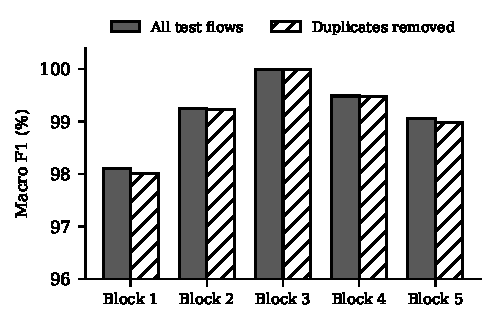
\includegraphics[width=\columnwidth]{figures/fig5_blocked.pdf}
\caption{Time-blocked evaluation of M1 on the corrected data.}
\label{fig:blocked}
\end{figure}

\textit{Two SSH flows.} The two SSH brute-force flows, one from each lab file, are far too few to estimate a detection rate. M1 labels both as SSH-Bruteforce, with confidence 0.82 and 0.78, and M0 labels both as DoS-Hulk, an attack label of the wrong class. We report them only as a check that M1 does not label everything benign. Both come from one attacker and one victim in one lab, and each is a single long connection.

\subsection{LIME again, with the retrained model}
RQ3 left one question open. LIME failed on most real flows with M0 and the original background. With M1 available, we asked whether the failure came from the background or from the kernel width. We first expected that a background drawn from the corrected data would help, so we ran LIME with M1 and a background of 2,000 corrected training flows on the same 313 real flows. With the kernel width of 3.312 that we had locked in RQ2, all 313 flows have an effective sample size below two, and none reaches the quality gate (Fig.~\ref{fig:lime}a and b). We then widened the kernel from 3.312 to 30,000 (Fig.~\ref{fig:lime}c). With M1, the number of flows that reach the gate rises to 136 at width 30, 265 at 300, 304 at 3,000, and 313 at 30,000. From width 300 on, the weights of the perturbed samples are almost equal, with a median effective sample size of 999 to 1,000 out of 1,000, so the fit approaches a global linear model of the classifier near the background and is no longer local. With M0 and the original background, widening helps much less, and 41 of 313 flows reach the gate at width 30,000. Passing the gate at a wide kernel therefore does not show that LIME explains the flow locally. We did not vary the number of perturbed samples. TreeSHAP values also passed the additivity check on all 784 flows for M1, with a largest error of $3.8\times 10^{-6}$.

\begin{figure*}[t]
\centering
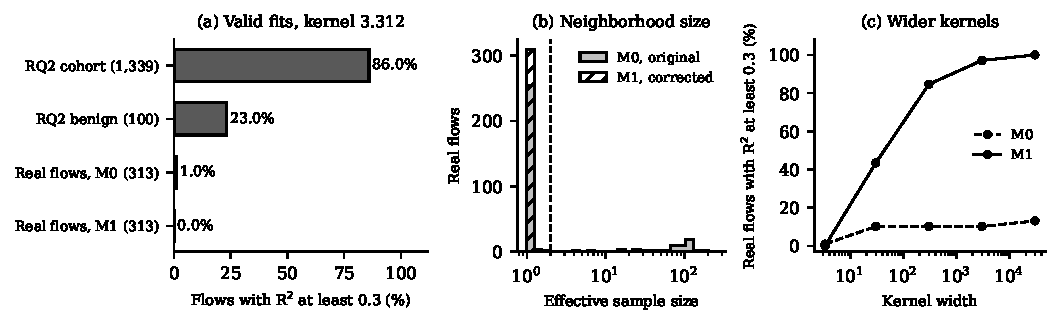
\includegraphics[width=0.92\textwidth]{figures/fig6_lime.pdf}
\caption{Validity of LIME explanations. (a) Share of explanations with a local fit of $R^2\ge 0.3$ at the locked kernel width of 3.312. (b) Effective sample size of the perturbed samples on the 313 real flows at that width. Values below two make the fit invalid. (c) Share of the 313 real flows that reach $R^2\ge 0.3$ as the kernel width grows.}
\label{fig:lime}
\end{figure*}

\textit{Answer to RQ4.} Yes for the first part. SHAP, a decision-path trace, and feature-intervention tests tied the failure to a three-condition region around the FIN flag count, and that region holds only Hulk flows in the original training data. Retraining on the corrected data removes the failure on our benign flows, but the corrected benchmark is easy, and the cause of the shortcut remains a hypothesis.

\section{Discussion and Limitations}
We separate the conclusions into three levels.

\textit{What the data show.} M0 uses a region of the feature space that holds only DoS-Hulk flows in its training data, and this region contains almost all of its false alerts on the live flows and on the labeled benign test flows. A SHAP chart of the false alerts pointed to the FIN count, and a decision-path trace turned that into three conditions. The retrained model M1 raises no alert on the 784 live flows and the 21 browsing flows.

\textit{What the data support but do not prove.} The shortcut most likely comes from an extractor that ended flows at the first FIN packet. Our evidence is the zone content of the training data, the difference in FIN frequency, and earlier reports on the extractor. We did not check the extractor on raw packets. The feature-intervention tests show how sensitive the model is to a feature, and they do not show what real traffic looks like.

\textit{What remains open.} Whether M1 detects attacks in a real network is unknown, because our attack evidence is two SSH flows. M1 replaces the FIN pattern with a header-size pattern that also depends on the operating system, and its benchmark contains near-duplicate flows. We do not report M1 on the original domain. LIME with other numbers of perturbed samples or with discretized features was not tested.

The data are limited in other ways. The live set comes from one laptop in four sessions, its benign label rests on our own statement without an activity log, and flows within a session are correlated. We left out other lab captures whose labels we could not verify. We tested only XGBoost and one corrected dataset. The reliability flags of the system are unvalidated, and we ran no study with analysts.

A practical rule follows from the case. Before deployment, run the classifier on a small set of benign traffic from the target network and inspect the explanation of each false alert.

\section{Conclusion}
We built an online intrusion detector in four steps. In RQ1, an XGBoost classifier reached 97.9\% accuracy on CSE-CIC-IDS2018. In RQ2, SHAP proved more faithful and stable than LIME. In RQ3, the deployed classifier raised an alert on 19.0\% of 784 live flows that we confirmed as benign. In RQ4, SHAP values, a decision-path trace, and feature-intervention tests identified a three-condition region around the FIN flag count. That region covered 148 of the 149 alerts and 99.97\% of the false alerts on a large labeled benign set, and in the original training data it held only DoS-Hulk flows. The data fit an extractor that ended flows at the first FIN, which we could not verify on raw packets. A classifier trained on the corrected data raised no alert on the live flows, but its benchmark is easy and its score should not be read as field performance. With the locked kernel width, LIME gave no valid fit on real flows, and wider kernels pass the quality gate only by making the fit nearly global, while TreeSHAP passed the additivity check on all of them. Future work should collect labeled attack traffic in a real network, check the extractor on raw packets, and test whether the reliability flags predict explanations that mislead analysts.

\appendices
\section{Data and Artifact Inventory}
Table~\ref{tab:inventory} lists the data, software, and seeds of the experiments. We did not record a version identifier for the corrected dataset, so the table gives only the date on which we obtained it.

\begin{table}[h]
\caption{Data, software, and seeds.}
\label{tab:inventory}
\centering
\footnotesize
\begin{tabular}{>{\raggedright\arraybackslash}p{0.95in}>{\raggedright\arraybackslash}p{2.1in}}
\toprule
Item & Value \\
\midrule
Original data & CSE-CIC-IDS2018 processed CSV files from the public AWS bucket. The 15,589,784 cleaned flows are in ten daily Parquet files \\
Corrected data & Recreated dataset of Liu et al., ten daily CSV files, obtained on 22 October 2026 \\
Flow extractor & Python CICFlowMeter 0.5.0 with project lifecycle version rq3-cfm-0.5.0-lifecycle-v3, Scapy 2.8.0, Npcap 1.89 \\
Software & Python 3.14.7, XGBoost 3.4.1, SHAP 0.52.0, LIME 0.2.0.1, scikit-learn 1.9.1, pandas 3.0.6 \\
Seeds & Split and XGBoost seed 42. Re-splits use seeds 1, 2, and 3. LIME uses a background of 2,000 flows drawn with seed 42 and a seed derived for each flow \\
\bottomrule
\end{tabular}
\end{table}

\balance
\bibliographystyle{IEEEtran}
\bibliography{refs}

\end{document}
